\documentclass[10pt, journal, compsoc]{IEEEtran}

\usepackage[pdftex]{graphicx}    
\usepackage{enumitem, mathtools, amssymb}
\usepackage[colorlinks=true, urlcolor=blue, linkcolor=blue]{hyperref}

\raggedbottom

\newcommand{\an}{AlexNet }
\newcommand{\gn}{GoogleNet }

\begin{document}
\title{Training Neural Networks for Robotic Inference}
\author{Stephan Hohne \thanks{S2H.Mobile@gmail.com}}

\markboth{Project 5, Robotics Software Engineer Nanodegree Program}%
{}
\IEEEtitleabstractindextext{%

\begin{abstract}
Two project tasks for object classification are carried out. First, a given data set containing images of grocery store items is used to create a model that meets criteria for inference time and accuracy. For the second task, image data for classification of three types of fruit is collected. For each task, the NVIDIA DIGITS GPU infrastructure is used to train a chosen neural network architecture for image classification. The resulting models are applied to infer the class of unknown data samples. The accuracy and time for inference is evaluated. Applications of these models to robotic systems such as object sorting on a conveyor belt are discussed.
\end{abstract}

\begin{IEEEkeywords}
Neural Network Training, Image Classification, Inference.
\end{IEEEkeywords}
}

\maketitle

\section{Introduction}
\label{sec:introduction}
\IEEEPARstart{D}{eep} neural networks with convolution layers have become a standard tool for object classification  \cite{geron}. Originally, they were used for recognizing handwritten digits, with the classic MNIST data set \cite{lecun-98}. The \an \cite{NIPS2012_4824} and \gn \cite{DBLP:journals/corr/SzegedyLJSRAEVR14} architectures were trained on the larger ImageNet data set. These deep neural networks rely on a large database of labeled samples, and are able to detect a variety of objects in images. 

In this project, classification of objects on a conveyor belt is studied. Two different tasks are specified.
\begin{description}
\item[Task 1] Classify grocery items on the conveyor belt in one of three categories \texttt{Bottle}, \texttt{Candy\_Box}, or \texttt{Nothing}.
\item[Task 2] Classify food items on the conveyor belt in one of three categories \texttt{apricot}, \texttt{egg}, or \texttt{tomato}.
\end{description}

The training data for the first task are provided in the Udacity workspace. The data set consists of $10094$ color images in PNG format. The training data for the second task is collected by taking pictures with an iPhone 6, resulting in $507$ color images in JPG format. 

The model training is performed using a GPU powered NVIDIA DIGITS environment, which also provides standard network architectures with  predefined hyperparameter settings. For the first task, the \an architecture \cite{NIPS2012_4824} is employed for model training. For the second task, \an \cite{NIPS2012_4824} and \gn \cite{DBLP:journals/corr/SzegedyLJSRAEVR14} are used.

This report is organized as follows. In section \ref{sec:background}, the choice and configuration of network architectures for this project is discussed. In section \ref{sec:data_acquisition}, the acquisition of image data and the training of the networks is described. The inference results of the trained models are stated in section \ref{sec:results} and discussed in section \ref{sec:discussion}. A conclusion and an outlook to future work is given in section \ref{sec:conclusion_future_work}.

\section{Background: Neural Networks for Classification}
\label{sec:background}
In order to accomplish the given object recognition tasks, the \an and \gn architectures were chosen for model training. The \an architecture  \cite{NIPS2012_4824} won the 2012 ImageNet challenge, where it achieved a $17 \%$ top-5 error rate \cite{geron}. The \gn architecture \cite{DBLP:journals/corr/SzegedyLJSRAEVR14} won the ILSRVC 2014 challenge, with a top-5 error rate below  $7 \%$ \cite{geron}. It features inception modules which allow for a much more efficient use of parameters. \gn uses $10$ times fewer parameters than \an which reflects in the model size. The proven performance of these architectures makes them good choices for attempting the given classification tasks. The NVIDIA DIGITS environment provides these architectures to the user, implemented using the \href{http://caffe.berkeleyvision.org/}{Caffe} framework.

\subsection{Task 1}
The model training was performed using the \an architecture over six episodes. The batch size was kept to network defaults. The stochastic gradient descent solver was used. The hyperparameter settings for the learning rate were kept at their default values. This means that the initial learning rate was $0.01$ for episodes one and two, $0.001$ for episodes three and four, and $0.0001$ for episodes five and six.

\subsection{Task 2}
For the task of food item classification, training was performed on two different network architectures, \an \cite{NIPS2012_4824} and \gn \cite{DBLP:journals/corr/SzegedyLJSRAEVR14}. For both architectures, the same parameter setting was used. the number of episodes was set to $30$. The batch size was kept at network defaults, and the stochastic gradient descent solver was used.  The hyperparameter settings for the learning rate were kept at their default values. This means that the initial learning rate was $0.01$ for the first ten episodes, $0.001$ for the next ten episodes, and $0.0001$ for the last ten episodes.

\section{Data Acquisition}
\label{sec:data_acquisition}
\subsection{Task 1}
The first project task was to practice the DIGITS workflow for model generation using a supplied data set. The raw training data is located in the workspace in the folder \texttt{/data/P1\_data}. The data set consists of $4568$ images in the class \texttt{Bottle}, $2495$ images of type \texttt{Candy\_Box}, and $3031$ images in the class \texttt{Nothing}, for a total of $10094$ color images. The files are in PNG format. Figure \ref{fig:default_dataset} shows the properties of the corresponding database creation job. The job was run with a train/val/test split of 60/20/20, so there were  $6057$ images for training, $2019$ images for validation and $2018$ images for testing. In order to match the size of the initial layer in the network, the images were squashed to a dimension of $256 \times 256$ pixels.

\begin{figure}[htpb]
      \centering
      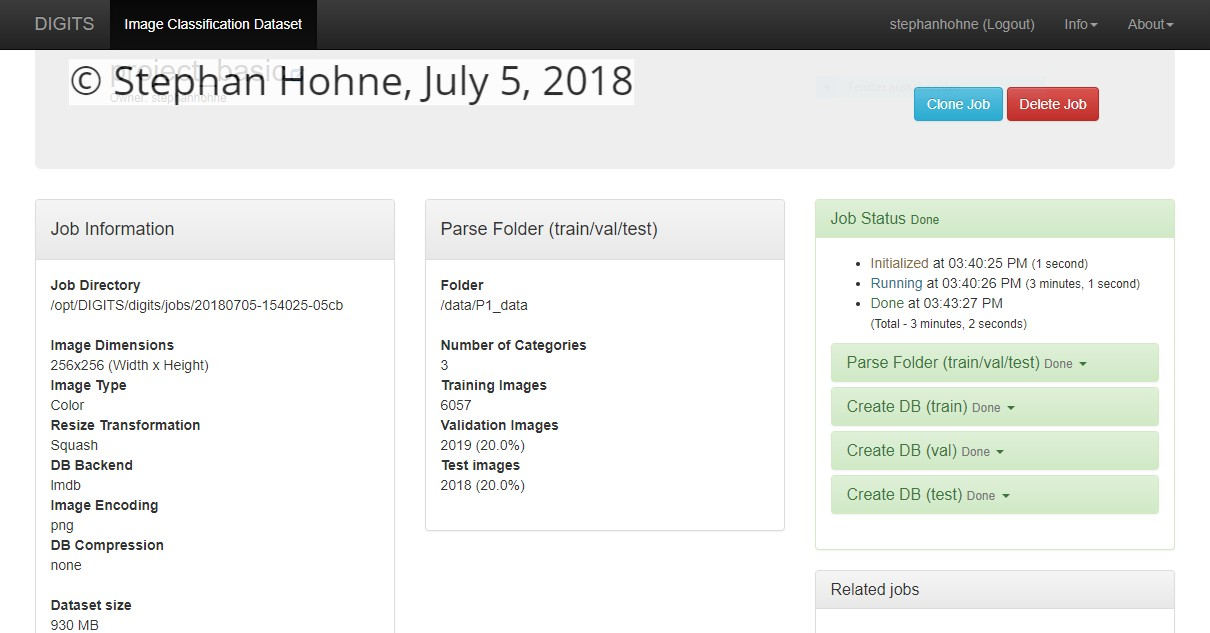
\includegraphics[width=\columnwidth]{images/default_dataset/dataset.PNG}
      \caption{Properties of database creation job 20180705-154025-05cb. Screenshot taken in the DIGITS environment.}
      \label{fig:default_dataset}
\end{figure}

\subsection{Task 2}
The training data for classifying food items was collected by taking pictures with an iPhone 6. The items were placed on a desk with a surface structure that resembles a conveyor belt. A variation in orientation and lighting was achieved by rotating the camera. In total, $507$ color images in JPG format were created. The image dimensions are $2448 \times 3264$, and each file has a size of approximately $2 - 3$ MB. There are $159$ images of eggs, $166$ images of apricots, and $182$ images of tomatoes used for training. The picture folders can be downloaded from Google Drive as shared files for \href{https://drive.google.com/file/d/1HW1X9KxycGZRnXoJ5xLPJWkrDRKEih3V/view?usp=sharing}{eggs}, \href{https://drive.google.com/file/d/1ugdK5Q70PKQ7CYgqdEBu2u8pBz-67MMZ/view?usp=sharing}{tomatoes}, and \href{https://drive.google.com/file/d/14c-oQIlffO4MASaPsXZYFmt2CiP5Hi8y/view?usp=sharing}{apricots}. Example images are shown in figures \ref{fig:IMG_1482}, \ref{fig:IMG_1565}, \ref{fig:IMG_1714}.

\begin{figure}[htpb]
      \centering
      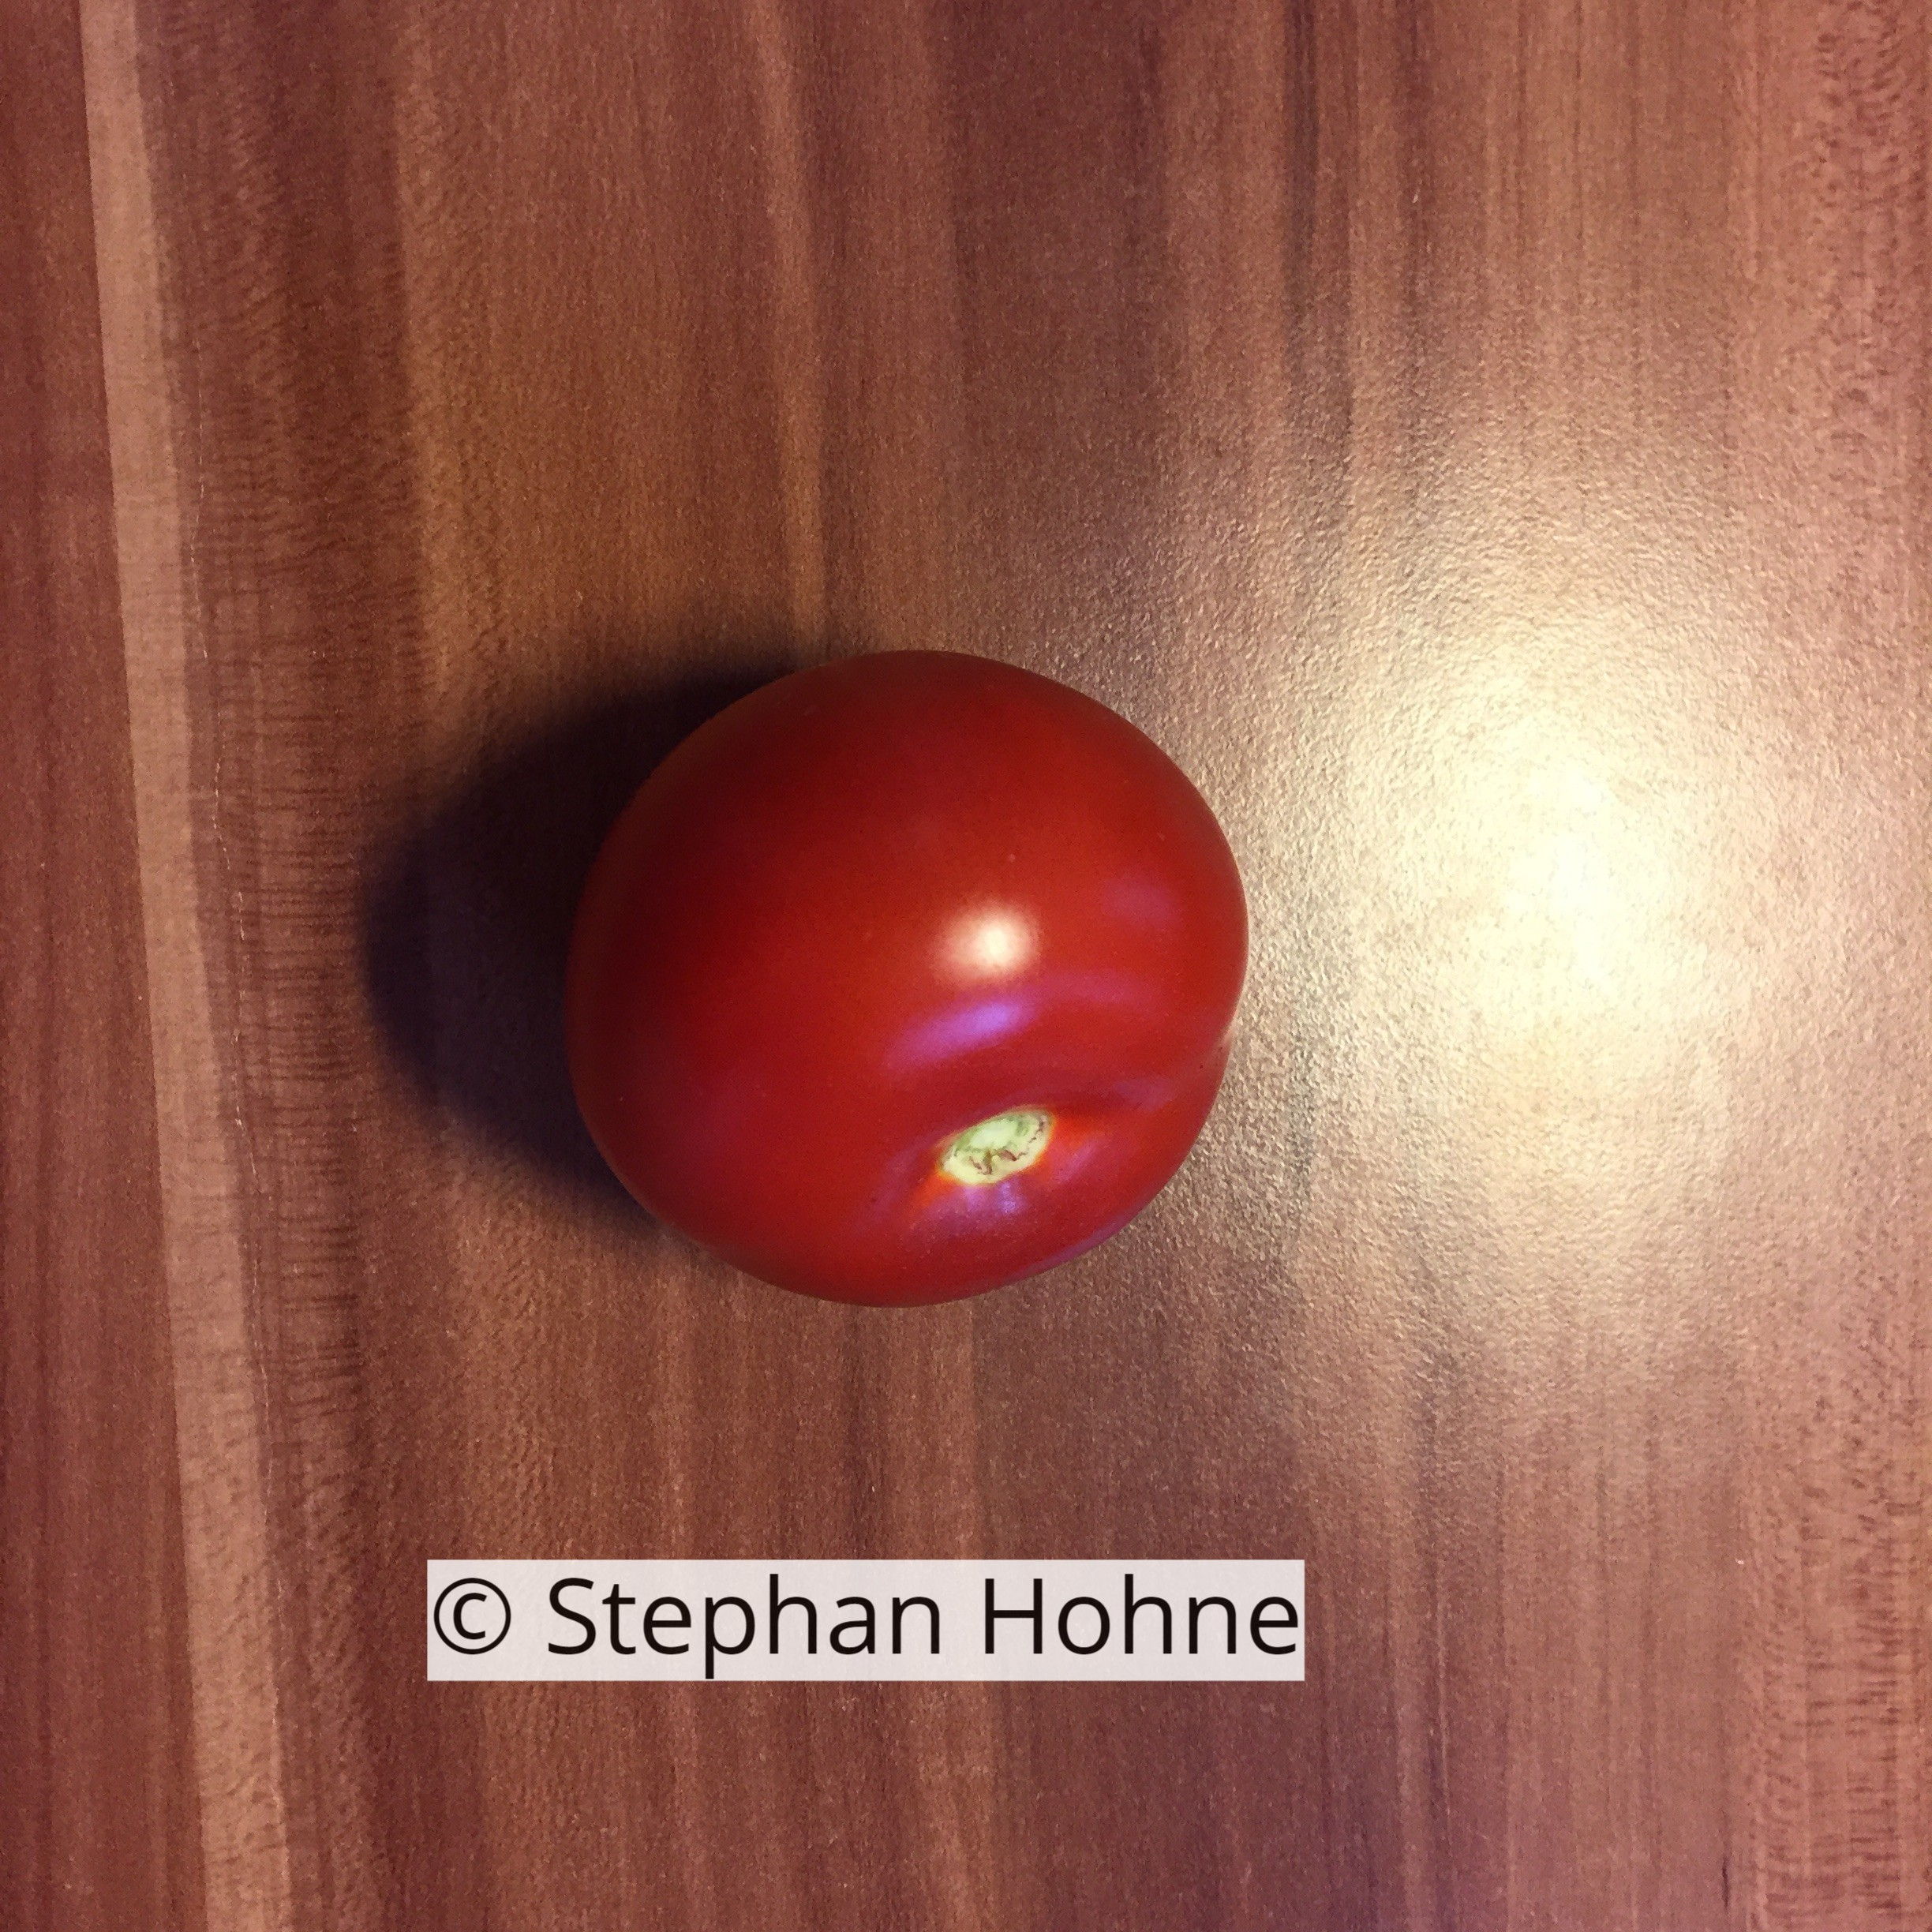
\includegraphics[width=\columnwidth]{images/data_samples/IMG_1482.jpg}
      \caption{Example image of a tomato in the training data set.}
      \label{fig:IMG_1482}
\end{figure}
\begin{figure}[htpb]
      \centering
      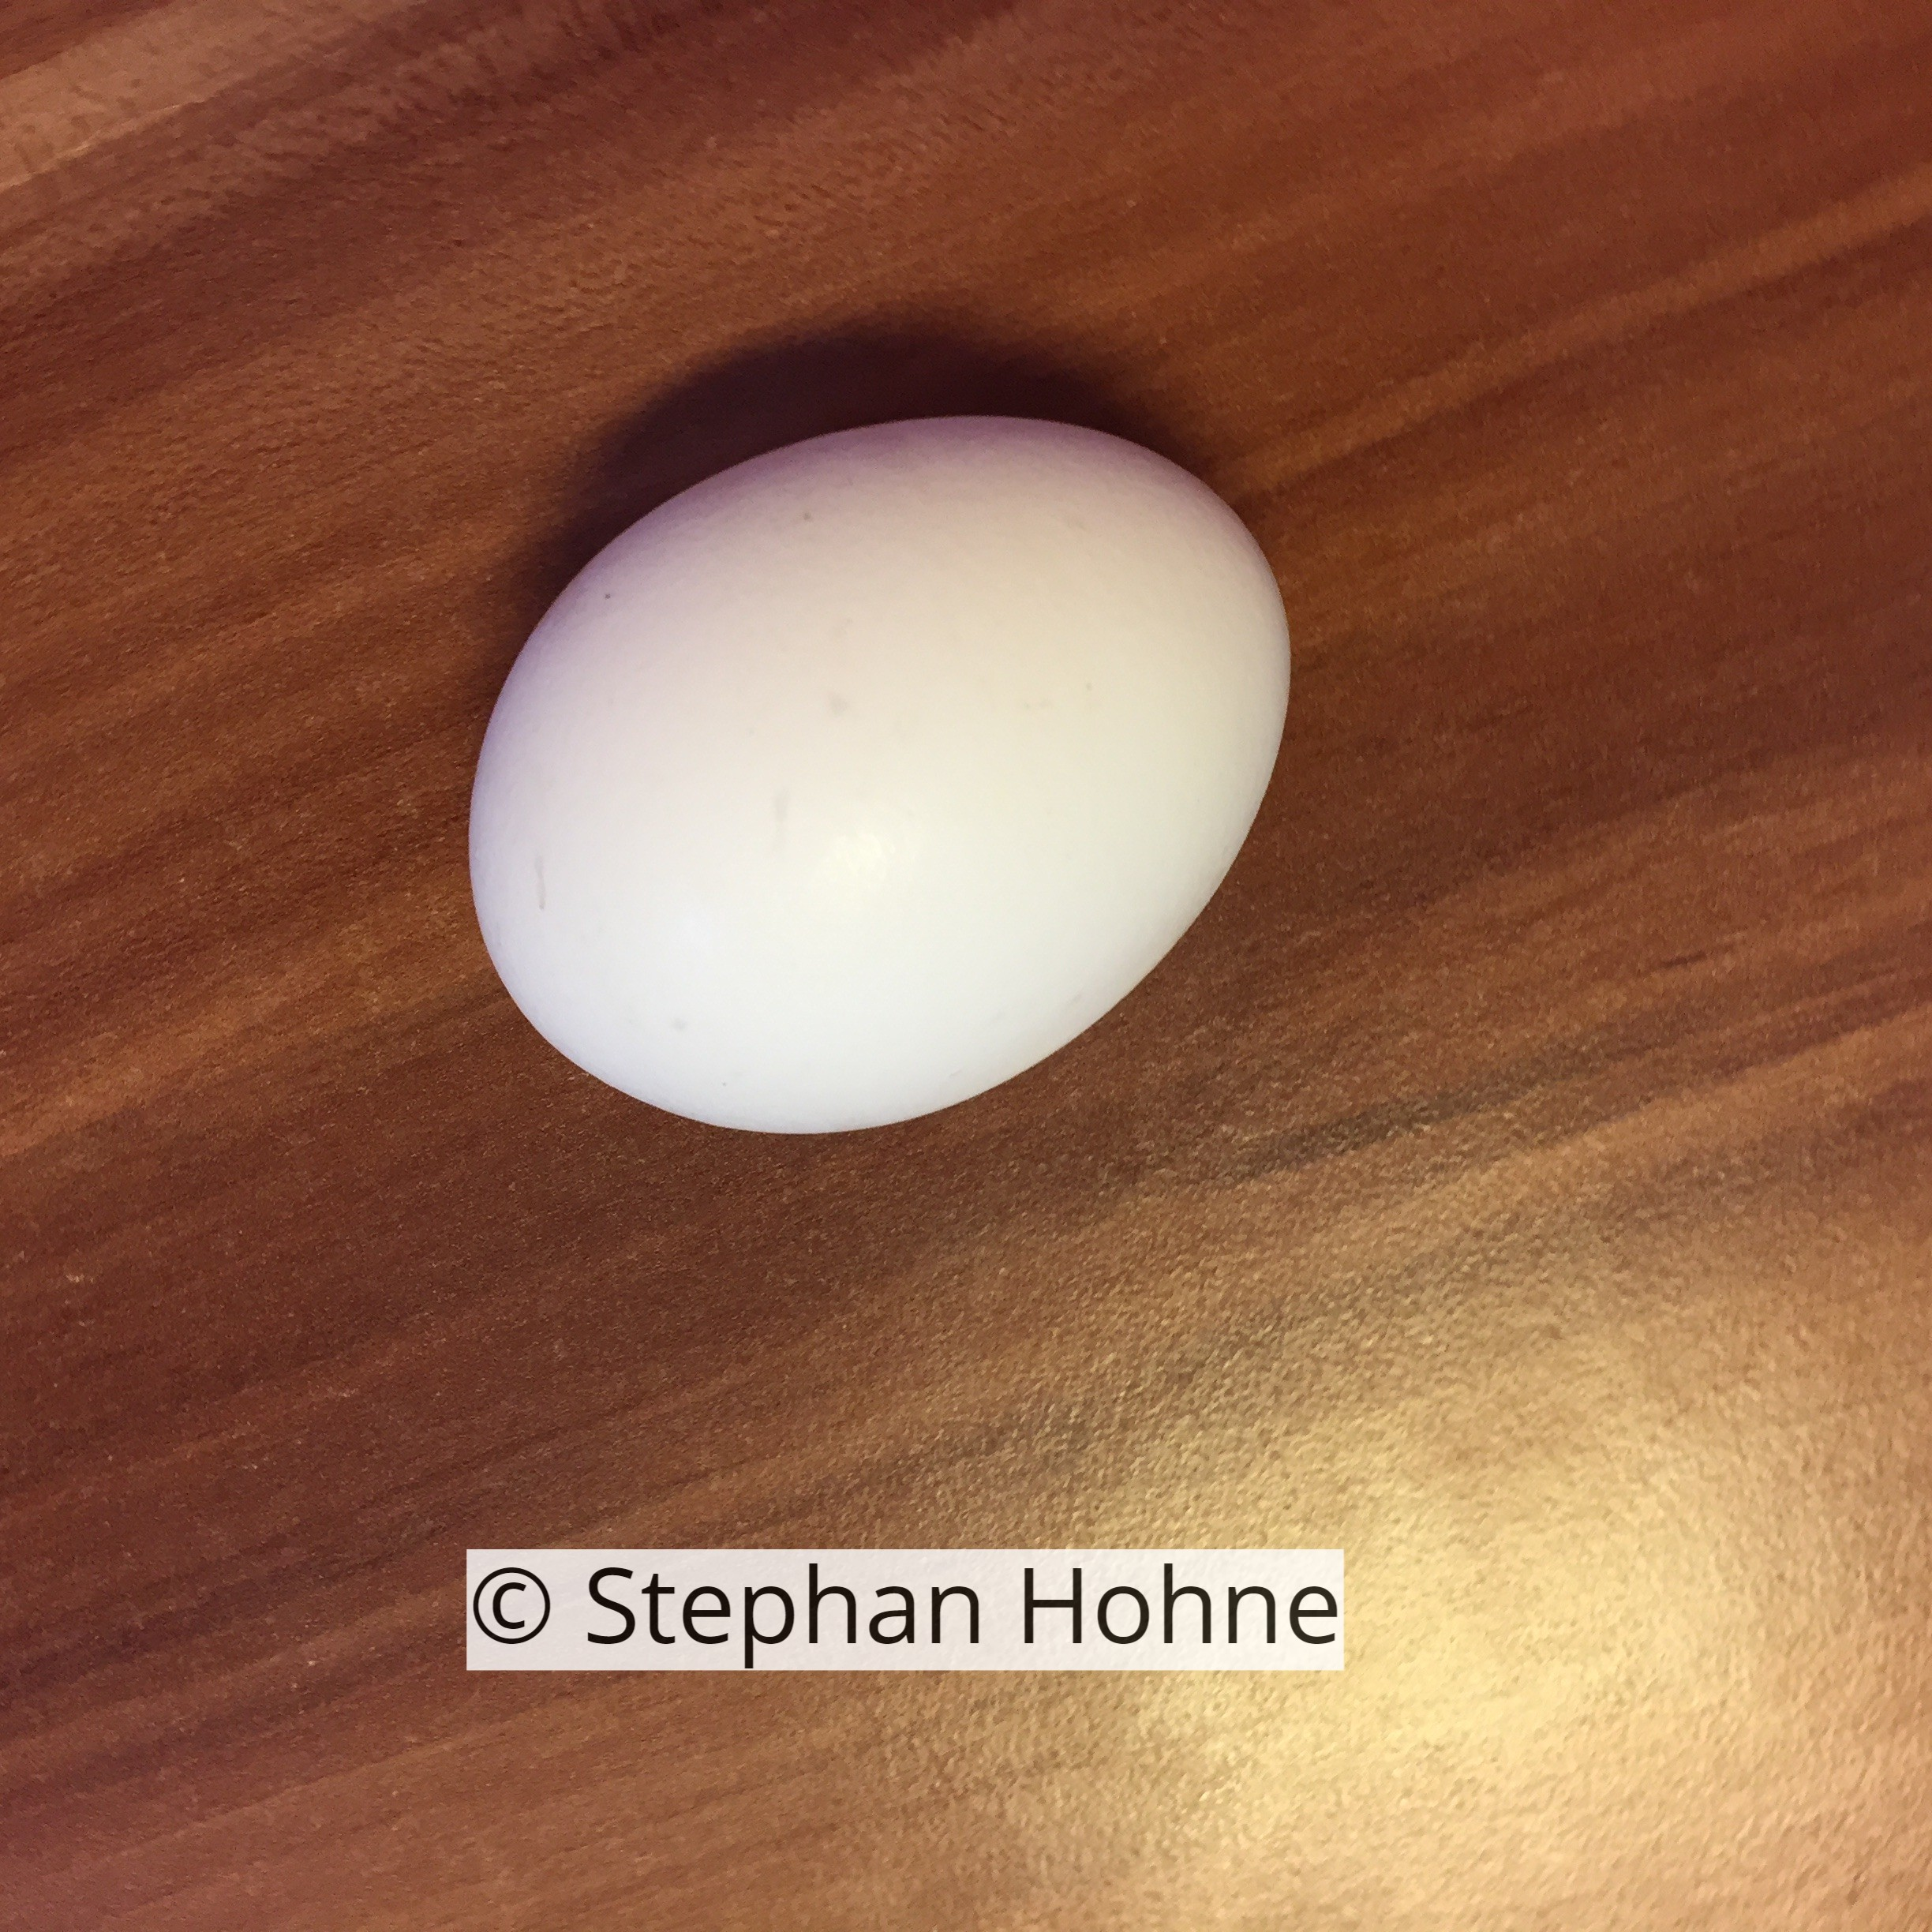
\includegraphics[width=\columnwidth]{images/data_samples/IMG_1565.jpg}
      \caption{Example image of an egg in the training data set.}
      \label{fig:IMG_1565}
\end{figure}
\begin{figure}[htpb]
      \centering
      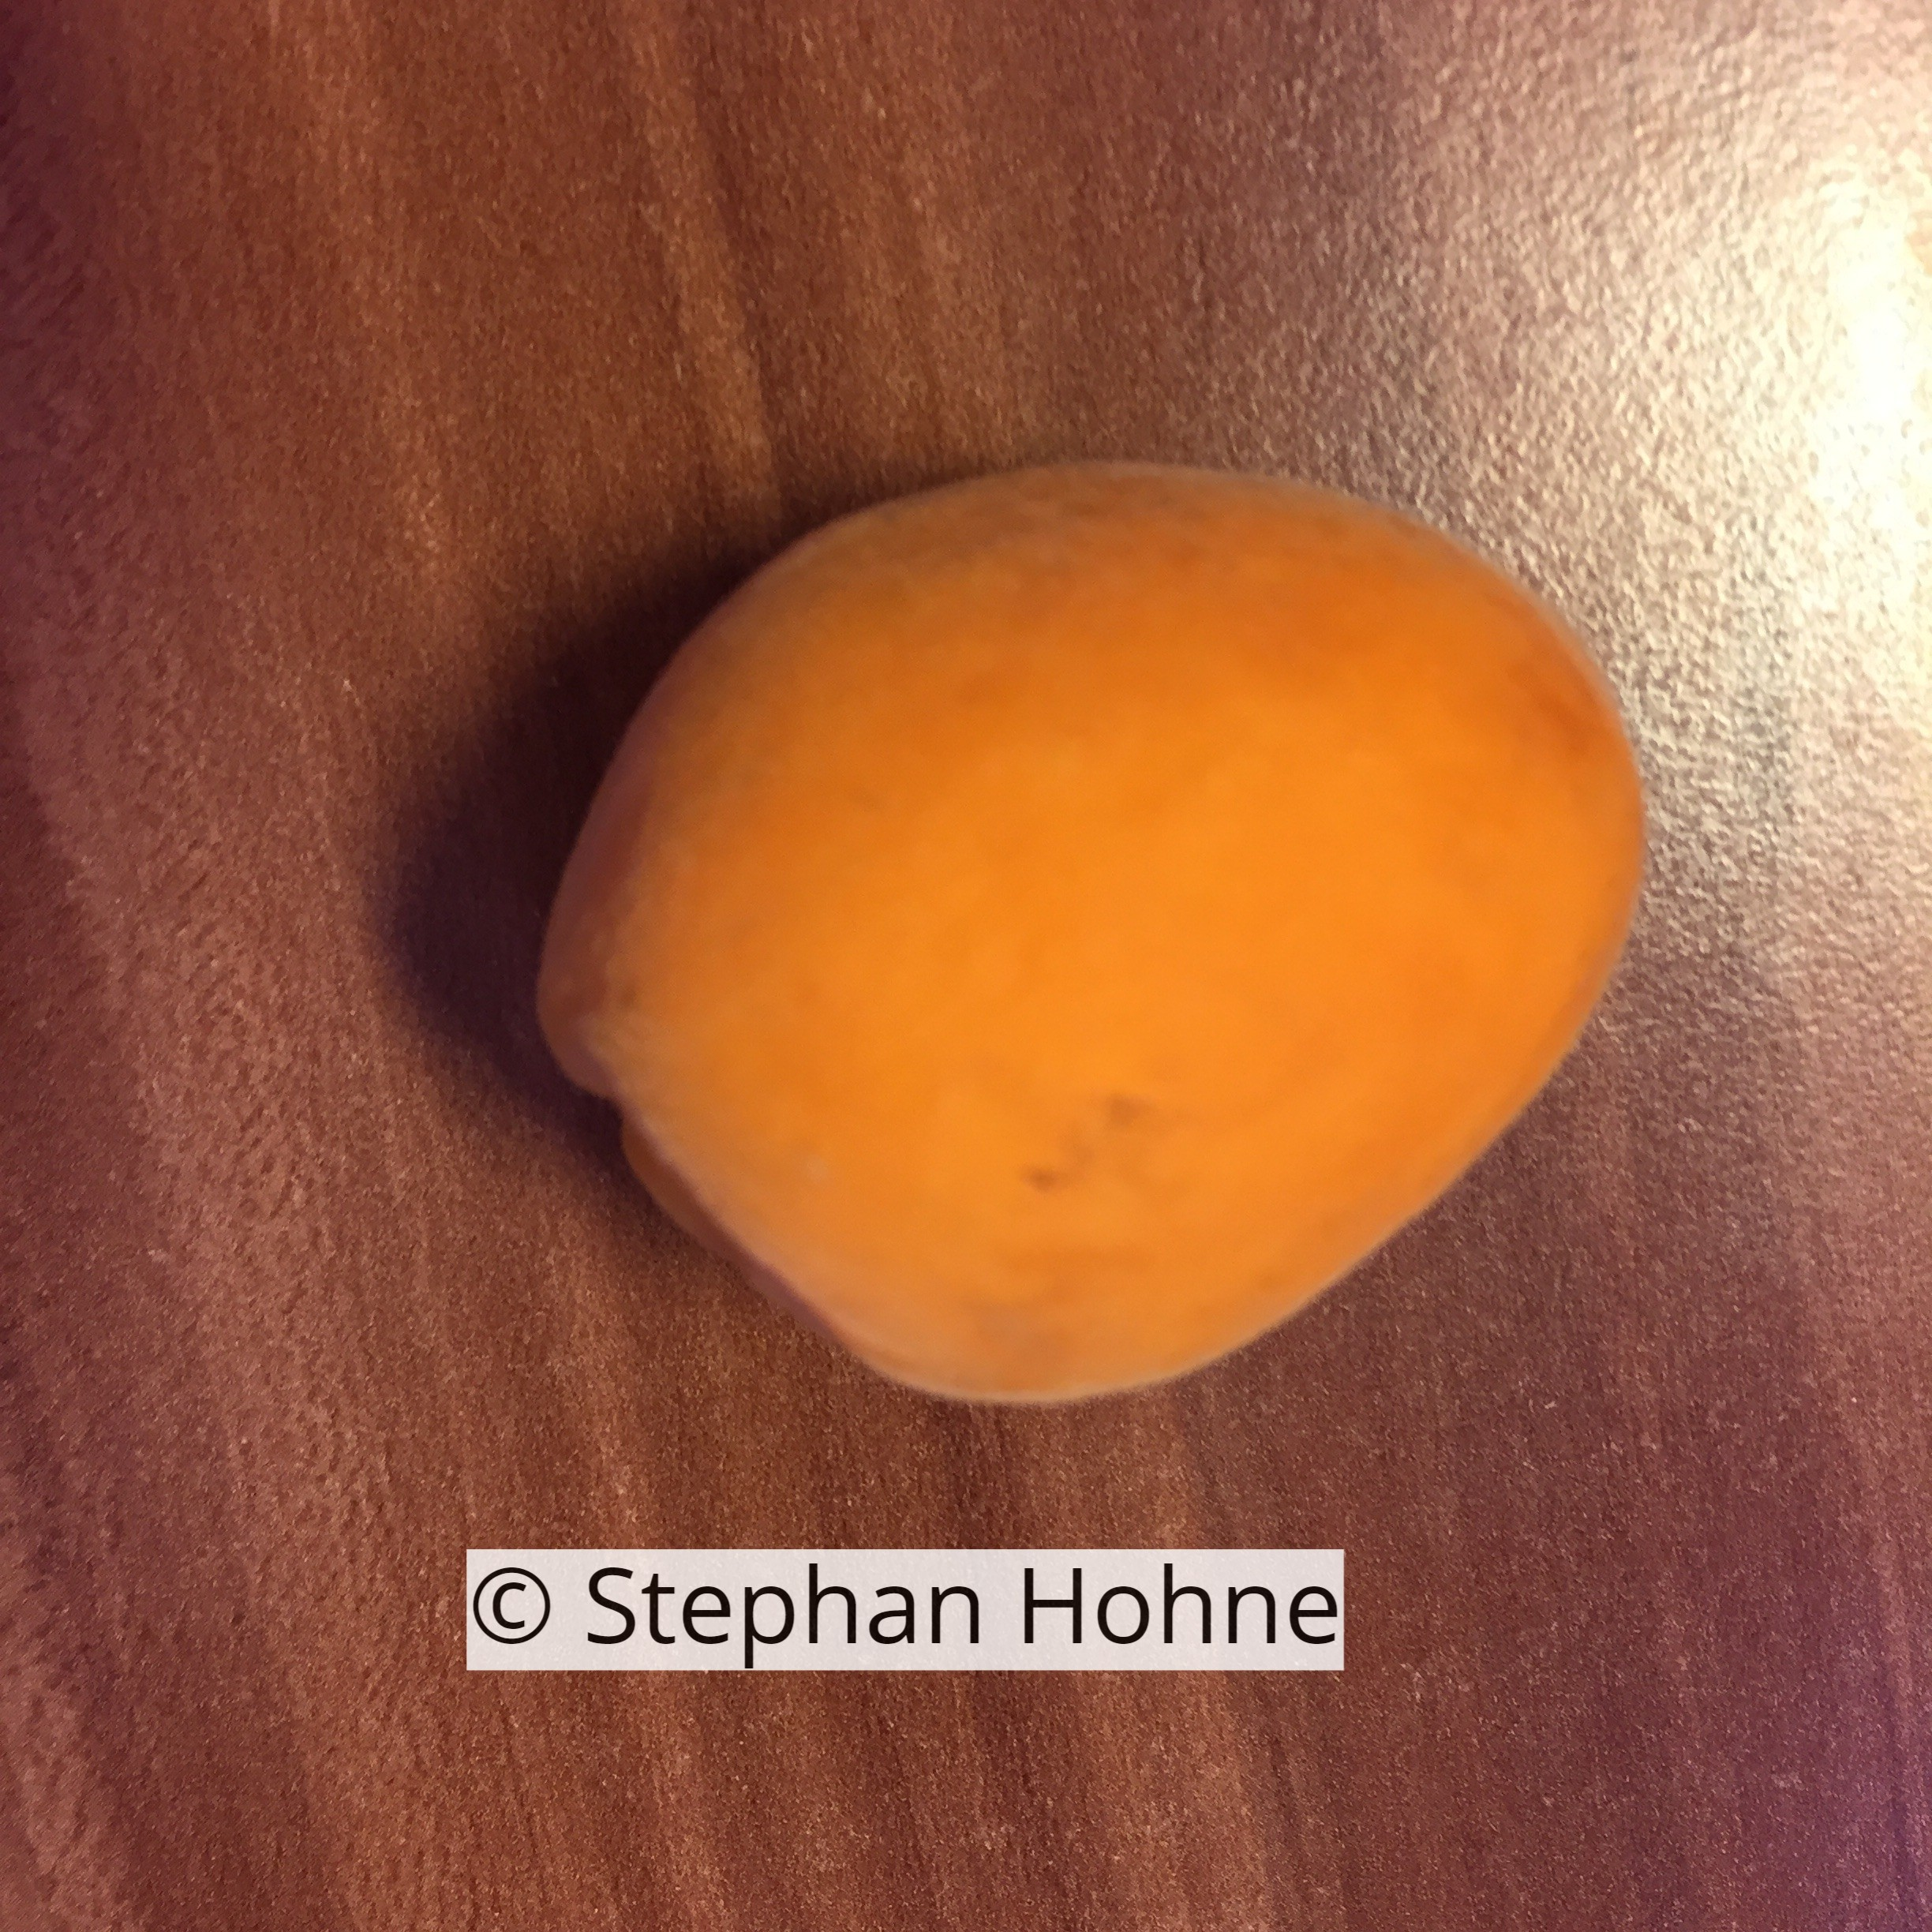
\includegraphics[width=\columnwidth]{images/data_samples/IMG_1714.jpg}
      \caption{Example image of an apricot in the training data set.}
      \label{fig:IMG_1714}
\end{figure}

The images used for inference were created in the same way. The inference data set consists of $11$ images of food items that are not present in the training data, $3$ pictures of an apricot, $4$ images of a tomato, and $4$ images of an egg. The inference images can be found in the \texttt{data/inference} folder in the project archive.

The database creation job was run with a train/val/test split of 60/20/20, so there were  $304$ images for training, $101$ images for validation and $102$ images for testing. In order to match the size of the initial layer in the network, the images were squashed to a dimension of $256 \times 256$ pixels.

\section{Results}
\label{sec:results}
\subsection{Task 1}
The model 20180705-160040-e827 resulted from training the \an architecture with the parameter setting described in section \ref{sec:background} on the data set described in section \ref{sec:data_acquisition}. The corresponding model files can be found in the \texttt{models/} folder in this archive. Since the \an architecture was used, the\texttt{.caffemodel} file is about $222$ MB in size.

\begin{figure*}[htpb]
      \centering
      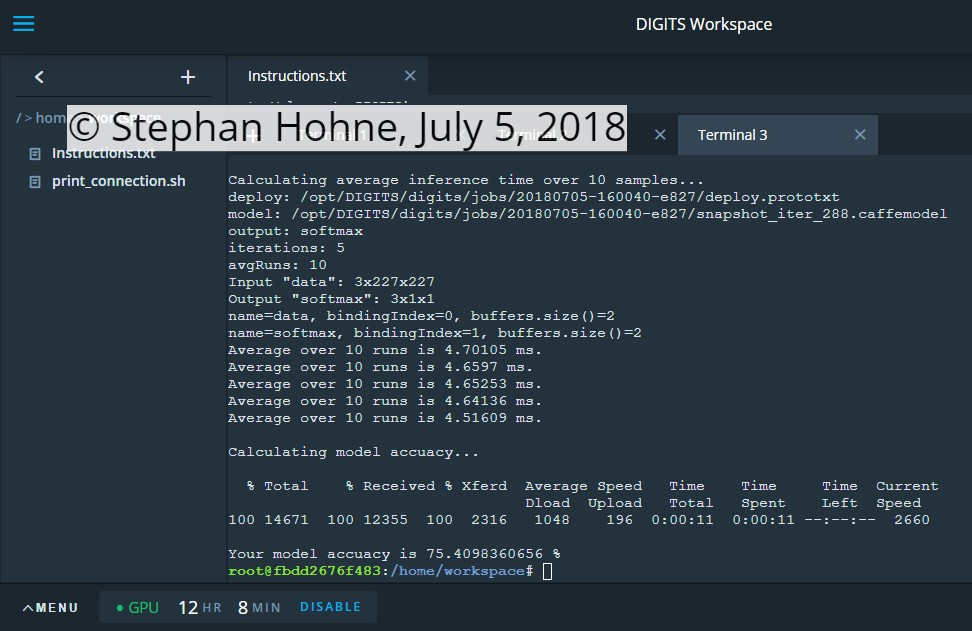
\includegraphics[width=\textwidth]{images/default_dataset/evaluation.PNG}
      \caption{Performance of model 20180705-160040-e827 on data set 20180705-154025-05cb. Output from the \texttt{evaluate} command. Screenshot taken in the Udacity workspace.}
      \label{fig:evaluation}
\end{figure*}

Figure \ref{fig:evaluation} shows the inference performance of this model as determined by using the \texttt{evaluate} command. The average inference time  is approximately $4.6 ms$. The accuracy is approximately $75.41\%$.

\subsection{Task 2}
The data set used for inference can be found in folder \texttt{/data/inference}. The corresponding image list can be found in the file \texttt{data/inference.list}. Both the \an and the \gn architectures were trained, as described in section \ref{sec:background}. This resulted in two different models named \texttt{new\_alex\_30} and \texttt{new\_large\_google\_30}. Each model achieved an accuracy of over $80\%$ on the inference data set. Since the \texttt{evaluate} command could not be applied to models generated with custom data, the inference time could not be measured. The performance of both models is summarized in table \ref{tab:performance}.

\begin{table}[htpb]
\caption{Accuracy of the models performing task 2.}
\label{tab:performance}
\begin{center}
\renewcommand{\arraystretch}{1.3}
\begin{tabular}{|l|c|c|}
\hline
Model & \texttt{new\_alex\_30} &\texttt{new\_large\_google\_30} \\
Screeenshot & \ref{fig:20180707-143126-1d4a_inference}& \ref{fig:20180707-144622-eca5_inference} \\
\hline
apricot  & $100\%$ &  $100\%$ \\
tomato   &  $50\%$ &  $50\%$  \\
egg      & $100\%$ & $100\%$ \\
\hline
total   & $81.8\%$  &  $81.8\%$\\
\hline
\end{tabular}
\end{center}
\end{table}

The models can be downloaded from Google Drive as shared files \href{https://drive.google.com/file/d/1zU4CfHpNheldrA8mJpPxxSZZS4ccLhVd/view?usp=sharing}{\texttt{new\_alex\_30}}, \href{https://drive.google.com/file/d/1mXt7rjXCMxZOcso7pLWbNrA-efT7cA7X/view?usp=sharing}{\texttt{new\_large\_google\_30}} in \texttt{tar.gz} format.

\section{Discussion}
\label{sec:discussion}
Both task 1 and task 2 involve classifying objects on a moving conveyor belt. The robotic inference project (task 2) is to sort food items, which could be commercially applied in logistics to package items separately. For both task 1 and task 2, the accuracy of classification is more important than the inference time. The rate of speed of the conveyor belt can be adjusted to the inference time. If necessary, the belt can be slowed down, which means that a smaller number of items can be sorted per time unit. This is more tolerable than incorrectly packaged food items. A classification model with longer inference time and higher accuracy should be preferred over a model with lower accuracy and shorter inference time. 

The models trained for task 2 seem to perform reasonably well at inferring the object classes. For applying these models to real conveyor belts, their accuracy needs to be improved further.

\begin{figure}[htpb]
      \centering
      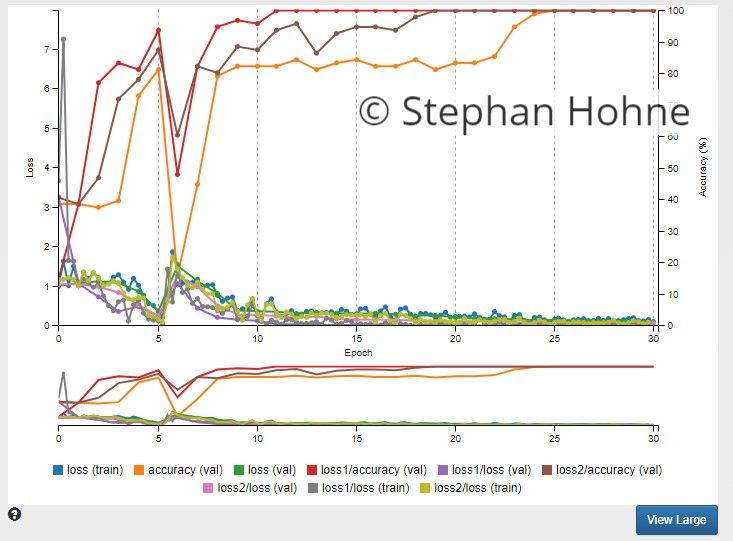
\includegraphics[width=\columnwidth]{images/training_curves/20180707-133949-aae5_training.PNG}
      \caption{Training curve over $30$ episodes for the model \texttt{large\_google\_30} with job id 20180707-133949-aae5.}
      \label{fig:20180707-133949-aae5_training}
\end{figure}

\begin{figure}[htpb]
      \centering
      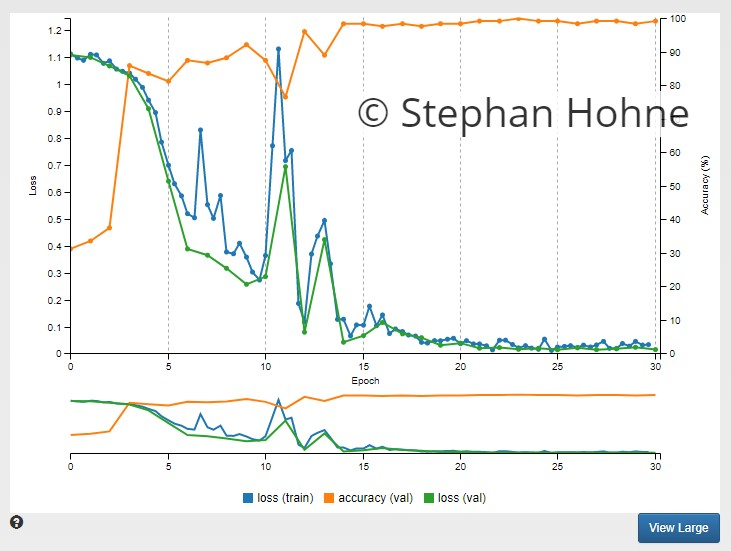
\includegraphics[width=\columnwidth]{images/training_curves/20180707-143126-1d4a_training.PNG}
      \caption{Training curve over $30$ episodes for the model \texttt{new\_alex\_30} with job id 20180707-143126-1d4a.}
      \label{fig:20180707-143126-1d4a_training}
\end{figure}

\begin{figure}[htpb]
      \centering
      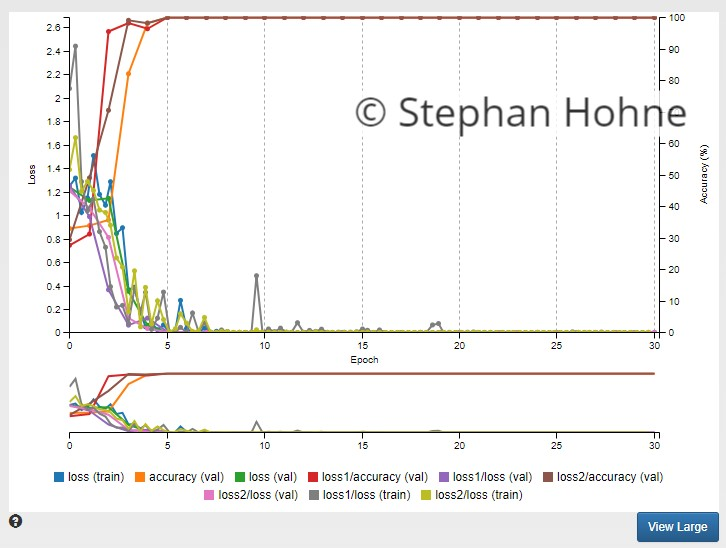
\includegraphics[width=\columnwidth]{images/training_curves/20180707-144622-eca5_training.PNG}
      \caption{Training curve over $30$ episodes for the model \texttt{new\_large\_google\_30} with job id 20180707-144622-eca5.}
      \label{fig:20180707-144622-eca5_training}
\end{figure}

The training curves shown in figures \ref{fig:20180707-133949-aae5_training}, \ref{fig:20180707-143126-1d4a_training} and \ref{fig:20180707-144622-eca5_training} indicate that the models over fit the training data, since the accuracy goes up to almost $100\%$ after only a few episodes. Since the networks and hyperparameters used for creating the models are proven standard, the main reason seems to be the limited amount of data collected. Therefore the main challenge when improving model performance is to collect more training data with a greater variety in lighting conditions, object orientation, etc.

Several methods of collecting image data were investigated. A laptop camera and the onboard camera of the Jetson TX2 were used. Variation in the images was achieved by moving the objects in between the snapshots. This method turned out to be inaccurate and inefficient, so that a large number of images could not be acquired in a reasonable amount of time. Moving the camera of a mobile phone instead of the object was more efficient.

\section{Conclusion and Future Work}
\label{sec:conclusion_future_work}
Two object classification tasks were performed. In the first task, the \an architecture was trained on a given data set and achieved an average inference time of about $4.6 ms$ and an accuracy of about $75.41\%$ at classifying grocery items on a conveyor belt. For the second task, image data of three types of food were collected, and used to train \an and \gn networks. The resulting models achieved overall accuracy of $80.0\%$, albeit on a small data set.

In order to deploy the models on a commercially viable product, more training data needs to be collected, which increases the accuracy and overall performance of the models. The choice of award wining architectures is a safe starting point for hyperparameter tuning. Therefore future work should include the following tasks.
\begin{itemize}
\item Collect more image data with a greater variety, possibly in an automated procedure.
\item Develop a means to determine the inference time fro custom models, where the \texttt{evaluate} command can not be applied.
\item Evaluate the models further. Create the confusion matrix. Calculate precision, recall and F1 score.
\item Explore the hyperparameter space of the convolution architectures. For instance, use the AdaGrad solver instead of stochastic gradient descent.
\item Deploy the inference models on the Jetson TX2. Mount the Jetson over a conveyor belt.
\end{itemize}

\begin{figure*}[thpb]
      \centering
      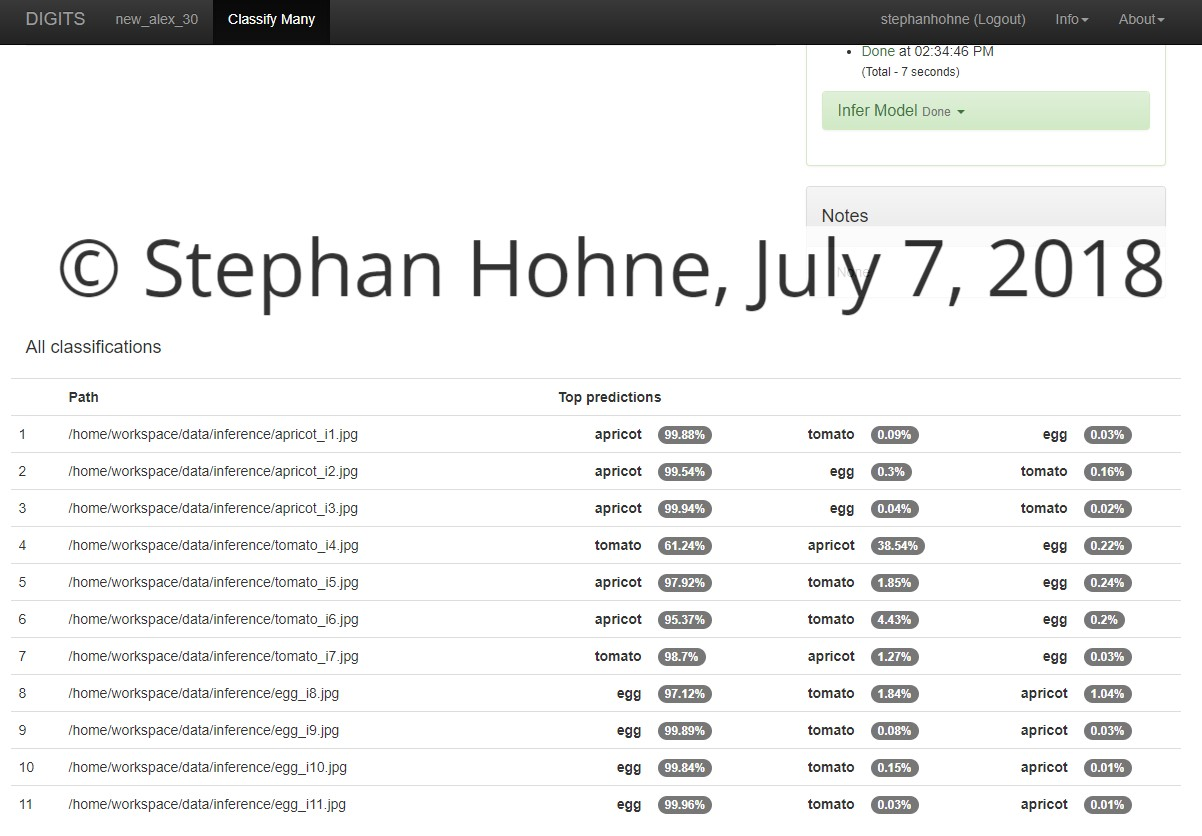
\includegraphics[width=\textwidth]{images/inference_results/20180707-143126-1d4a_inference.PNG}
       \caption{Inference results for the model \texttt{new\_alex\_30} with job id 20180707-143126-1d4a. Screenshot taken in the DIGITS workspace.}
      \label{fig:20180707-143126-1d4a_inference}
\end{figure*}
\begin{figure*}[thpb]
      \centering
      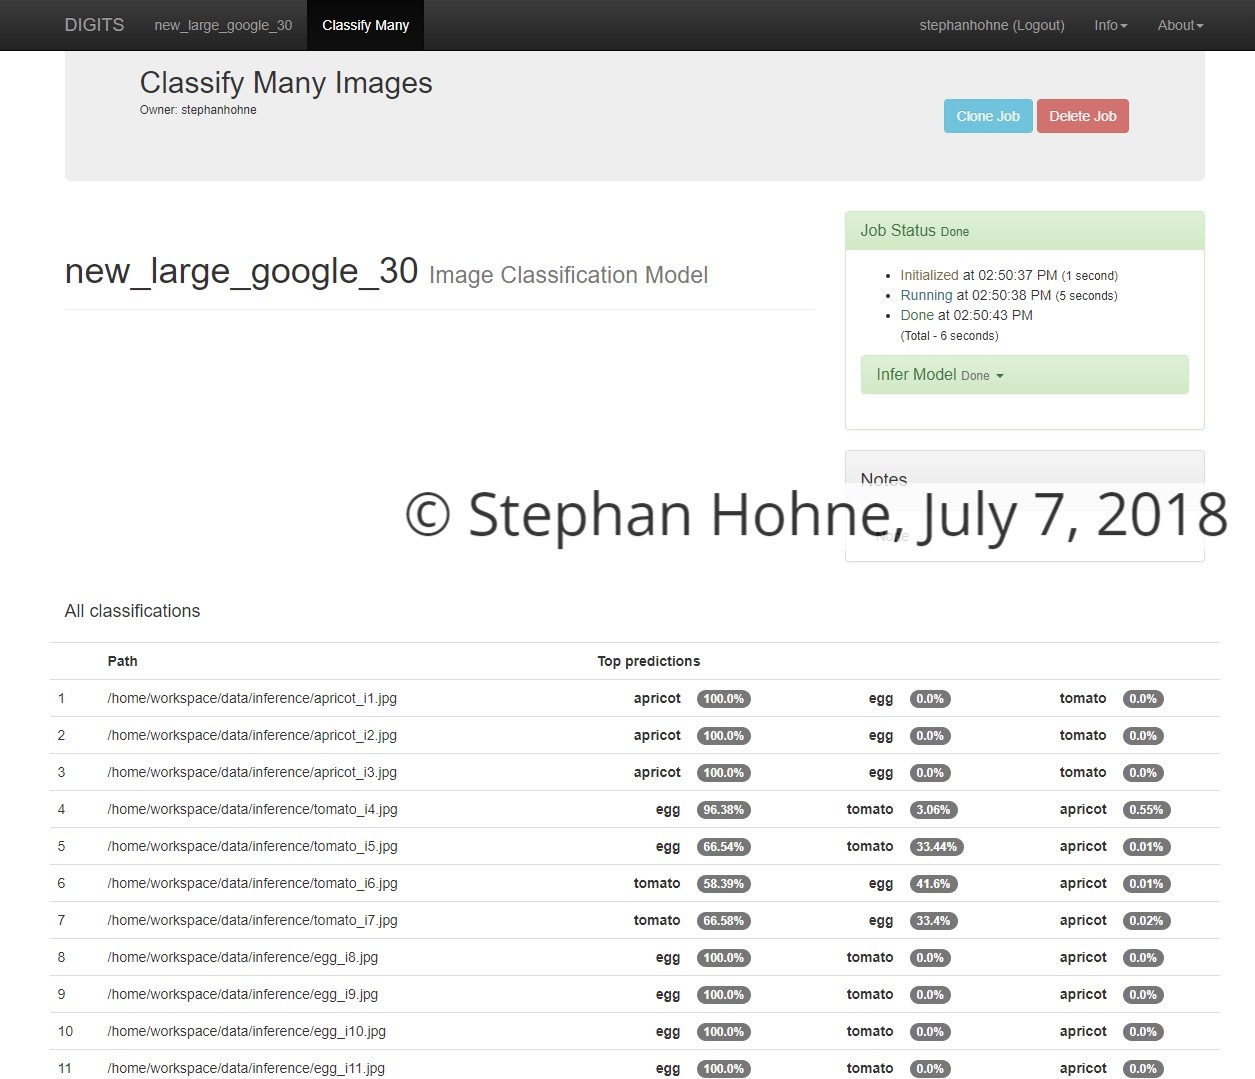
\includegraphics[width=\textwidth]{images/inference_results/20180707-144622-eca5_inference.PNG}
      \caption{Inference results for the model  \texttt{new\_large\_google\_30} with job id 20180707-144622-eca5. Screenshot taken in the DIGITS workspace.}
      \label{fig:20180707-144622-eca5_inference}
\end{figure*}


\bibliography{bib}
\bibliographystyle{ieeetr}

\end{document}